\documentclass[14pt,utf8,notheorems,compress,t]{beamer}
\usepackage{etex}

\usepackage[english]{babel}

\RequirePackage[all]{xy}
\usepackage{mathtools}
\usepackage{booktabs}
\usepackage{array}
\usepackage{ragged2e}
\usepackage{multicol}
\usepackage{tabto}
\usepackage{xstring}

\usepackage[protrusion=true,expansion=true]{microtype}

\setlength\parskip{\medskipamount}
\setlength\parindent{0pt}

\renewcommand{\U}{\mathcal{U}}
\newcommand{\NN}{\mathbb{N}}
\newcommand{\id}{\mathrm{id}}
\newcommand{\ZZ}{\mathbb{Z}}
\newcommand{\RR}{\mathbb{R}}
\newcommand{\Id}{\mathrm{Id}}
\newcommand{\fst}{\mathsf{fst}}
\newcommand{\snd}{\mathsf{snd}}
\newcommand{\inv}{\mathsf{inv}}
\newcommand{\refl}{\mathsf{refl}}
\newcommand{\ap}{\mathsf{ap}}
\renewcommand{\succ}{\mathsf{succ}}
\newcommand{\seg}{\mathsf{seg}}
\newcommand{\base}{\mathsf{base}}
\newcommand{\lloop}{\mathsf{loop}}
\newcommand{\ua}{\mathsf{ua}}
\newcommand{\code}{\mathsf{code}}
\newcommand{\surf}{\mathsf{surf}}
\newcommand{\merid}{\mathsf{merid}}
\newcommand{\N}{\mathsf{N}}
\renewcommand{\S}{\mathsf{S}}
\newcommand{\Cyl}{\mathrm{Cyl}}
\newcommand{\IsContr}{\mathsf{IsContr}}
\newcommand{\IsMereProp}{\mathsf{IsMereProp}}
\newcommand{\IsSet}{\mathsf{IsSet}}
\newcommand{\IsEquiv}{\mathsf{IsEquiv}}
\newcommand{\LEM}{\mathsf{LEM}}
\newcommand{\UIP}{\mathsf{UIP}}
\newcommand{\fib}{\mathsf{fib}}
\newcommand{\List}{\mathsf{List}}
\newcommand{\defeq}{\vcentcolon=}
\newcommand{\defeqv}{\vcentcolon\equiv}
\newcommand{\ct}{%
  \mathchoice{\mathbin{\raisebox{0.5ex}{$\displaystyle\centerdot$}}}%
             {\mathbin{\raisebox{0.5ex}{$\centerdot$}}}%
             {\mathbin{\raisebox{0.25ex}{$\scriptstyle\,\centerdot\,$}}}%
             {\mathbin{\raisebox{0.1ex}{$\scriptscriptstyle\,\centerdot\,$}}}
}
\renewcommand{\_}{\mathpunct{.}}
\newcommand{\fix}{\mathsf{fix}}

\newtheorem{axiom}{Axiom}

\title{Double-negation translation and\\ CPS transformation}
\author{
  \texorpdfstring{
    \vspace{-1em} \\
    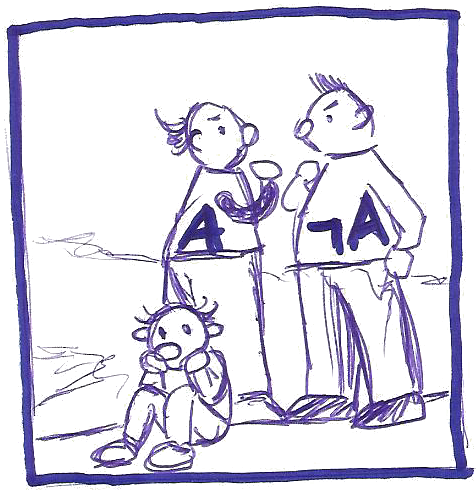
\includegraphics[scale=0.6]{lem} \\[0.5em]
    Ingo Blechschmidt \\[-0.3em]
    {\scriptsize June 3rd, 2015}%
  }{Ingo Blechschmidt}
}
\date{June 3d, 2015}

\usetheme{Warsaw}
\usecolortheme{seahorse}
%\usefonttheme{default}?
\usepackage[T1]{fontenc}
\usepackage{libertine}
\usefonttheme{serif}
%\usepackage{libertine}?
%\usepackage{mathpazo}
\useinnertheme{rectangles}

\setbeamertemplate{title page}[default][colsep=-1bp,rounded=false,shadow=false,bg=white]
\setbeamertemplate{frametitle}[default][bg=red,colsep=-2bp,rounded=false,shadow=false,center]
\setbeamertemplate{blocks}[rounded][shadow=false]

\setbeamertemplate{frametitle}{%
  \vskip1em%
  \leavevmode%
  \begin{beamercolorbox}[dp=1ex,center]{}%
      \usebeamercolor[fg]{item}{\textbf{\textsf{\Large \insertframetitle}}}
  \end{beamercolorbox}%
}

\setbeamertemplate{footline}{%
  \leavevmode%
  \hfill%
  \begin{beamercolorbox}[ht=2.25ex,dp=1ex,right]{}%
    \usebeamerfont{date in head/foot}
    \insertframenumber\,/\,\inserttotalframenumber\hspace*{1ex}
  \end{beamercolorbox}%
  \vskip0pt%
}

\setbeamertemplate{headline}{}
\setbeamertemplate{navigation symbols}{}

\newcommand{\floatbox}[3]{%
  \raisebox{0pt}[0pt][0pt]{%
    \begin{picture}(0,0)(#1,#2)#3\end{picture}\leavevmode%
  }%
}

\newcommand{\backupstart}{
  \newcounter{framenumberpreappendix}
  \setcounter{framenumberpreappendix}{\value{framenumber}}
}
\newcommand{\backupend}{
  \addtocounter{framenumberpreappendix}{-\value{framenumber}}
  \addtocounter{framenumber}{\value{framenumberpreappendix}} 
}

\newcommand{\hil}[1]{{\usebeamercolor[fg]{item}{\textbf{#1}}}}

\newcommand{\img}[3]{\begin{center}\includegraphics[scale=#1]{#2}\\\scriptsize#3\end{center}}
%\newcommand{\imageslide}[3]{\frame{\frametitle{#1}\img{#2}{#3}}}

\IfSubStr{\jobname}{\detokenize{nonotes}}{
  \setbeameroption{hide notes}
}{
  \setbeameroption{show notes}
}
\setbeamertemplate{note page}[plain]

\newenvironment{changemargin}[2]{%
  \begin{list}{}{%
    \setlength{\topsep}{0pt}%
    \setlength{\leftmargin}{#1}%
    \setlength{\rightmargin}{#2}%
    \setlength{\listparindent}{\parindent}%
    \setlength{\itemindent}{\parindent}%
    \setlength{\parsep}{\parskip}%
  }%
  \item[]}{\end{list}}

\graphicspath{{images/}}

\begin{document}

\frame[plain,c]{
  \begin{center}
    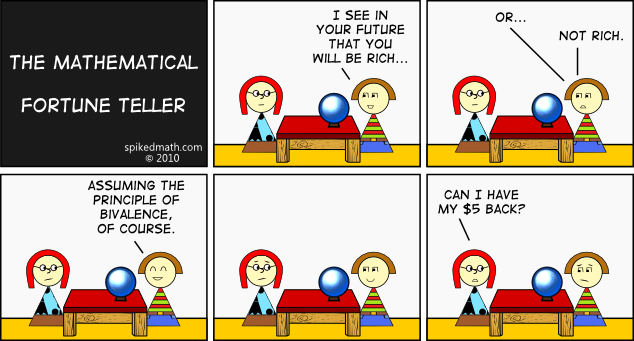
\includegraphics[scale=0.65]{fortune-teller}
  \end{center}
}

\frame{\titlepage}

\note{\fontsize{8pt}{9.6}\selectfont
  \begin{center}\large\textbf{Abstract}\end{center}

  \begin{changemargin}{2.5em}{2.5em}
    \justifying
    Constructive mathematicians don't use the law of excluded middle, which
    approximately says that for any proposition~$P$, either~$P$ is true or~$\neg P$
    is true. Several advantages emerge from this rejection, for instance one
    can mechanically extract algorithms from constructive proofs of existence
    statements and rigorously work with non-standard \emph{dream axioms} which are
    plainly false in classical mathematics, such as \emph{any function is
    smooth}.

    For communicating with classicial mathematicians, constructive
    mathematicians can employ the \emph{double-negation translation}. This
    device associates to any formula a translated formula in such a way that
    a given formula holds classically if and only if its translation holds
    constructively.

    The talk will give an introduction to these topics and discuss the
    intriguing relationship of the double-negation translation with the
    well-known con\-tin\-u\-a\-tion-pas\-sing style transformation: In some sense, they are
    the same. This is a beautiful facet of \emph{computational trinitarianism}.

    For the first part of the talk, no background in formal logic or
    constructive mathematics is required. For the second part of the talk,
    one should be vaguely familiar with the continuation-passing style
    transformation.
  \end{changemargin}
}

\frame{\frametitle{Outline}\begin{itemize}\item[]\tableofcontents\end{itemize}}

\section{Constructive mathematics}

\subsection{The law of excluded middle}

\newcommand{\constructiveinterpretation}{
  \begin{minipage}{0.99\textwidth}
    \begin{block}{\centering Constructive interpretation}
      \begin{description}\small
        \item[$\bot$] There is a contradiction.
        \item[$A \wedge B$] We have evidence for $A$ and for $B$.
        \item[$A \vee B$] We have evidence for $A$ or for $B$.
        \item[$A \Rightarrow B$] We can transform evidence for $A$ into
        one for $B$.
        \item[$\forall x{:}X\_ A(x)$] Given $x:X$, we can construct evidence
        for $A(x)$.
        \item[$\exists x{:}X\_ A(x)$] We have an $x:X$ together with evidence
        for $A(x)$.
      \end{description}
    \end{block}
  \end{minipage}
}

\frame{\frametitle{The law of excluded middle}
  \centering
  ``For any formula~$A$, we may deduce~$A \,\vee\, \neg A$.''

  \medskip
  Classical logic $=$ \\
  intuitionistic logic $+$ law of excluded middle.

  \vfill

  \only<1>{
    \begin{minipage}{0.8\textwidth}
      \begin{block}{\centering Classical interpretation}
        \begin{description}\small
          \item[$\bot$] There is a contradiction.
          \item[$A \wedge B$] $A$ and $B$ are true.
          \item[$A \vee B$] $A$ is true or $B$ is true.
          \item[$A \Rightarrow B$] If~$A$ holds, then also~$B$.
          \item[$\forall x{:}X\_ A(x)$] For all~$x:X$ it holds that~$A(x)$.
          \item[$\exists x{:}X\_ A(x)$] There is an $x:X$ such that~$A(x)$.
        \end{description}
      \end{block}
    \end{minipage}
  }
  \only<2>{
    \constructiveinterpretation
  }
  \par
}

\note{\justifying\footnotesize
  More precisely, one should say: Classical mathematics $=$ intuitionistic
  logic $+$ law of excluded middle $+$ a set theory including the axiom of
  choice.

  The constructive interpretation of the axiom of excluded middle is: For any
  formula~$A$, we have evidence for~$A$ or for~$\neg A$. This is an absurd
  statement.

  Several years ago a video showing Kate Moss consuming drugs surfaced.
  From the video it was clear that the drugs were either of some type~$A$ or of some type~$B$,
  but there was no direct evidence for either type.
  Kate Moss was not prosecuted; in this sense, Great Britain's judicial system
  operated intuitionistically.

  Note that constructive mathematicians do \emph{not} claim that the law of excluded
  middle is false (that is, that its negation holds). In fact, some
  instances of the law of excluded middle are true intuitionistically: For
  example one can show by induction that any natural number is zero or is not
  zero. Constructive mathematicians simply don't suppose that the law of
  excluded holds generally.
  \par
}

\subsection{Interpretation of intuitionistic logic}

\frame{\frametitle{Negated statements}
  \centering
  ``$\neg A$'' is syntactic sugar for $(A \Rightarrow \bot)$ \\[0.2em]
  and means: There can't be any evidence for~$A$.

  \vfill
  \constructiveinterpretation
  \par
}

\note{\justifying\footnotesize
  Note that the word ``contradiction'' is not generally forbidden in
  intuitionistic logic. For instance, the usual proof that~$\sqrt{2}$ is not
  rational, deducing~$\bot$ from the assumption that~$\sqrt{2}$ were rational,
  is perfectly fine intuitionistically.

  Colloquially, those proofs are called ``proof by contradiction'', but this
  labeling is deceptive. A true proof by contradiction runs like this:

  \begin{quote}We want to show~$A$. Assume~$\neg A$. Then $\ldots$,
  so~$\bot$. Therefore~$\neg\neg A$. Thus~$A$.\end{quote}

  The last step needs the axiom of double negation elimination, $\neg\neg A
  \Rightarrow A$, which is not available in intuitionistic logic. (In fact, the
  statement that double negation elimination holds for all~$A$ is equivalent to
  the statement that the law of excluded middle holds for all~$A$.)
  \par
}

\frame{\frametitle{Doubly-negated statements}
  \centering
  ``$\neg\neg A$'' means: There can't be any evidence for~$\neg A$.

  Trivially, we have $A \Longrightarrow \neg\neg A$. \\
  We can't deduce $\neg\neg A \Longrightarrow A$.

  \vfill
  \constructiveinterpretation
  \par
}

\note{\justifying
  If we know that the key to our apartment has to be somewhere in the
  apartment (since we used it to enter last night) but we can't find it, we can
  constructively only justify
  \[ \neg\neg \exists x\_ \text{the key is at position $x$}, \]
  not the stronger statement
  \[ \phantom{\neg\neg} \exists x\_ \text{the key is at position $x$}. \]
}

\subsection{Applications}

\frame{\frametitle{Applications}
  \begin{changemargin}{-0.5em}{-0.5em}
    \only<1>{
      \vspace*{-0.5em}
      Intuitionistic logic \ldots
      \begin{itemize}
        \item can guide to more elegant proofs, \\[0.2em]
        \item is good for the mental hygiene, and \\[0.2em]
        \item allows to make finer distictions.
      \end{itemize}
    }
    \only<2>{
      \begin{itemize}
        \item We can \hil{mechanically extract algorithms} from intuitionistic proofs
        of existence statements. \\[0.2em]
        \item The \hil{internal language of toposes} is intuitionistic.
        \\[0.2em]
        \item \hil{Dream mathematics} only works intuitionistically.
      \end{itemize}
    }
  \end{changemargin}

  \vfill
  \centering
  \only<1>{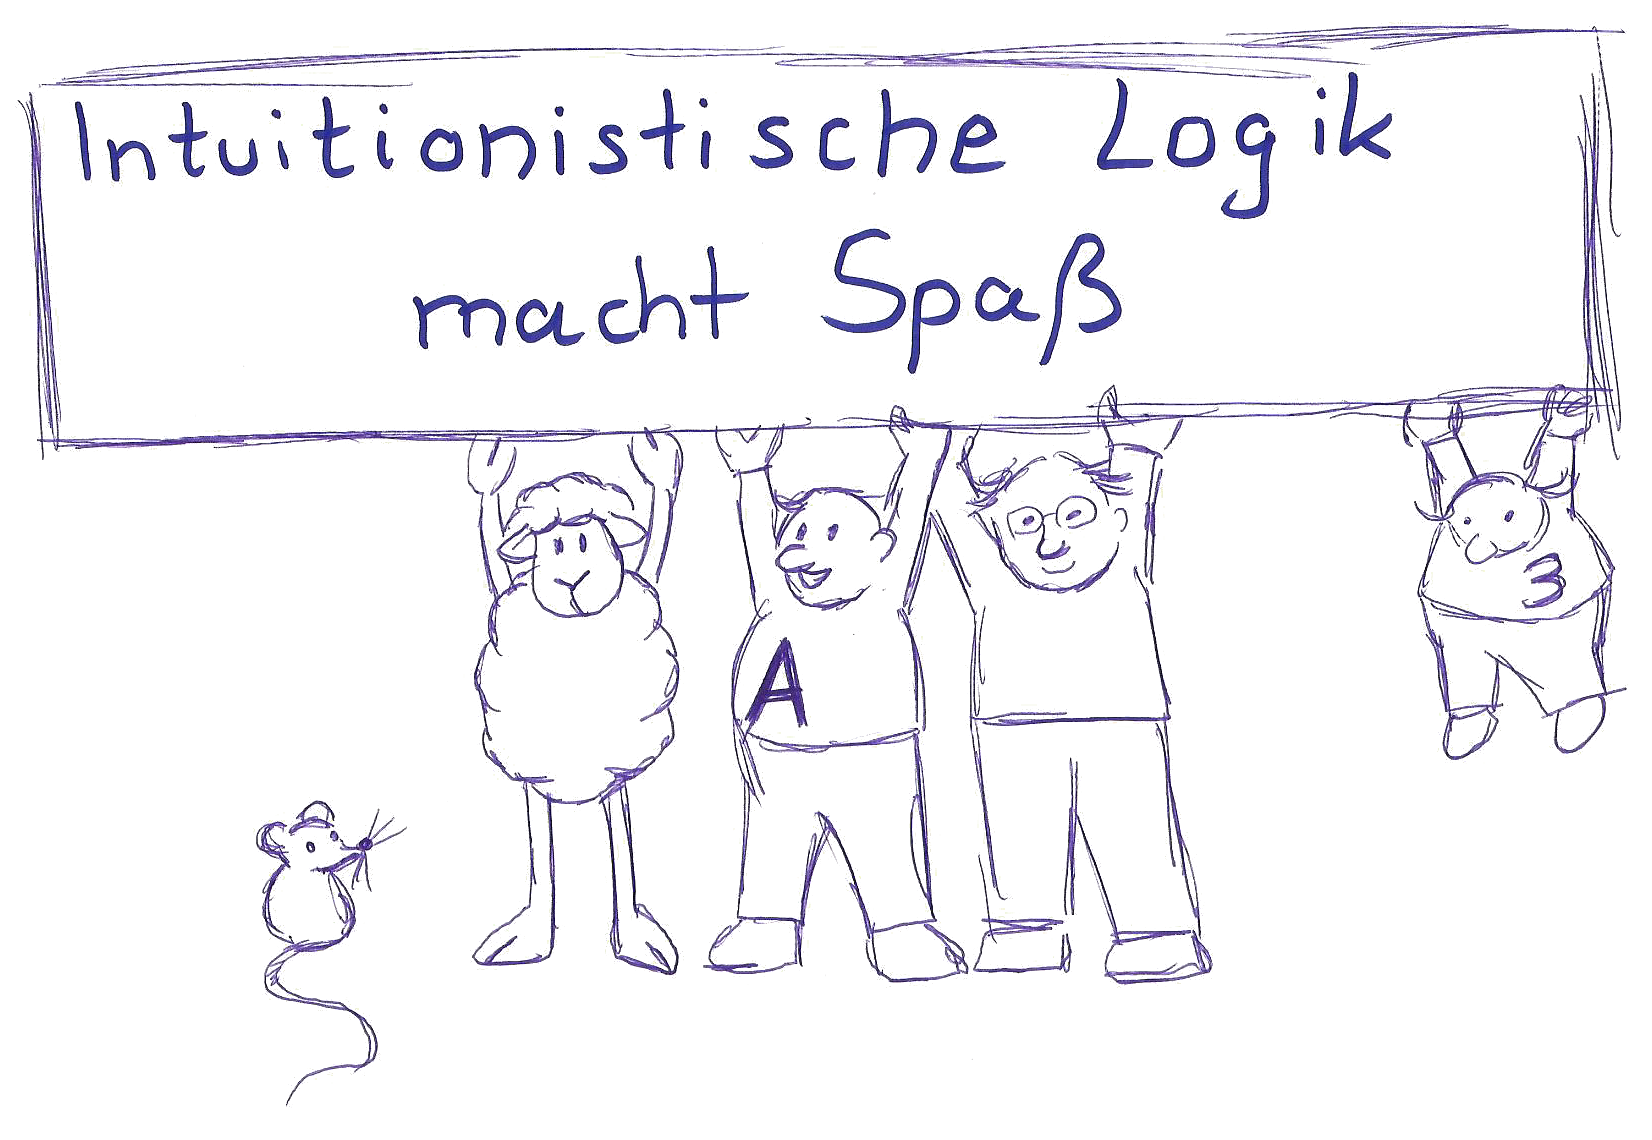
\includegraphics[height=5cm]{fun}}
  \only<2>{%
    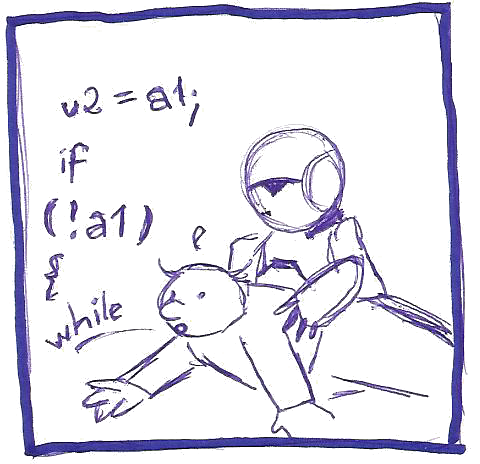
\includegraphics[height=3cm]{program-extraction}
    \hfill
    
\includegraphics[height=3cm]{constructive-maths}
    \hfill
    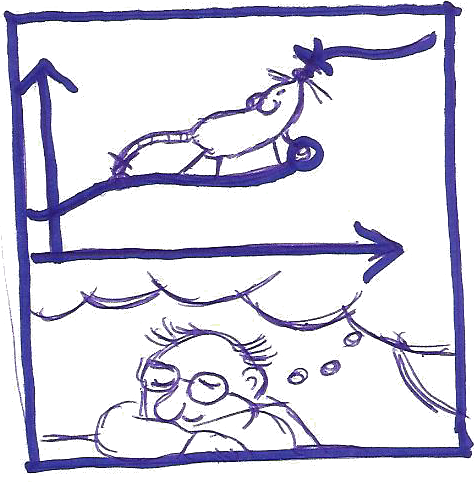
\includegraphics[height=3cm]{dream-maths}
  }
  \par
}

\note{\justifying\footnotesize
  Here is a basic example for extracting algorithms from proofs. Consider the
  statement

  \begin{quote}``There are infinitely many prime numbers.''
  \textnormal{or somewhat more explicitly,}
  ``For any finite list~$p_1,\ldots,p_n$ of prime numbers, there
  exists an additional prime number~$q$ not on that list.''\end{quote}
  The standard proof, attributed to Euclid, goes like this:

  \begin{quote}
  Consider the number~$N \defeq p_1 \cdots p_n + 1$.
  Since~$N \geq 2$, there exists some prime factor~$q$ of~$N$. (If~$N$ is
  itself prime, we can take~$q \defeq N$.)
  This prime is not equal to any~$p_i$, since the numbers~$p_i$ don't divide~$N$
  whereas~$q$ does.
  \end{quote}

  The algorithm for constructing~$q$ can be directly read off from the proof.
  Different proofs result in different algorithms; in particular, there exist
  (more complex) proofs whose algorithms produce better (smaller) witnesses.

  See the wonderful book \emph{Applied Proof Theory: Proof Interpretations and
  their Use in Mathematics} by Kohlenbach for details. Already its introduction
  is a very worthwhile reading.\par
}

\note{\justifying\footnotesize
  Tangentially, observe that the stated constructive version of Euclid's proof
  is less prone to misunderstandings than its well-known counterpart which uses
  proof by contradiction:

  \begin{quote}Assume that there are only a finite number of
  primes,~$p_1,\ldots,p_n$. Then consider~$N \defeq p_1 \cdots p_n +
  1$. This number is either prime or composite. Since no prime number
  divides~$N$ (by assumption the only primes are the~$p_i$ and these don't
  divide~$N$), it cannot be composite. Therefore~$N$ is prime. Since~$N$
  doesn't equal any of the~$p_i$, this is a contradiction.
  \end{quote}

  From this proof one might think that for primes~$p_1,\ldots,p_n$ the
  number~$N \defeq p_1 \cdots p_n + 1$ is always prime. But this only holds in
  a counterfactual world where there are only finitely many primes. In fact,
  the number
  \[ N \defeq 2 \cdot 3 \cdot 5 \cdot 7 \cdot 11 \cdot 13 + 1 = 59 \cdot 509 \]
  is composite. A shorter example is
  \[ N \defeq 2 \cdot 7 + 1 = 3 \cdot 5. \]
}

\frame{\frametitle{Topos power}
  \centering

  \begin{minipage}{0.65\textwidth}
    \begin{exampleblock}{}
      \justifying
      Any finitely generated vector space does \emph{not not} possess a basis.
    \end{exampleblock}
  \end{minipage}
  \medskip

  \scalebox{3}{$\Downarrow$}

  \begin{minipage}{0.65\textwidth}
    \begin{exampleblock}{}
      \justifying
      Any sheaf of modules of finite type on a \mbox{reduced} scheme is locally free on a dense
      open subset.
    \end{exampleblock}
  \end{minipage}
  \par
}

\note{\justifying\footnotesize
  Toposes are certain kinds of categories, thought of as \emph{mathematical
  universes}. The usual topos in which we do mathematics is the category of
  sets and maps between sets, but there are many others:
  \begin{itemize}
  \item In the \emph{effective topos}, any map is computable.
  \item In the \emph{sheaf topos} of a topological space~$X$ the objects and
  morphisms depend on our position in~$X$.
  \end{itemize}
  A metatheorem states that \emph{intuitionistically provable statements holds
  in any topos}. This greatly expands the scope of an intuitionistic theorem.

  A side project of mine is to recognize the basic concepts and statements of
  algebraic geometry as topos-theoretic interpretations of simple concepts and
  statements of ordinary first-year linear algebra. See
  \url{https://github.com/iblech/internal-methods} for expository notes on this
  topic.
  \par
}

\frame{\frametitle{Dream mathematics}
  \centering

  \begin{minipage}{0.85\textwidth}
    \begin{block}{\centering Synthetic differential geometry}
      Any map~$\RR \to \RR$ is smooth.
    \end{block}
  \end{minipage}

  \begin{minipage}{0.85\textwidth}
    \begin{block}{\centering Synthetic domain theory}
      \justifying
      For any set~$X$ there exists a map
      \vspace*{-0.9em}
      \[ \fix : (X \to X) \to X \]
      \vspace*{-2.1em}

      such that
      $f(\fix(f)) = \fix(f)$ for any~$f : X \to X$.
    \end{block}
  \end{minipage}

  \begin{minipage}{0.85\textwidth}
    \begin{block}{\centering Synthetic computability theory}
      \justifying
      There are only countably many subsets of~$\NN$.
    \end{block}
  \end{minipage}

  \par
}

% XXX:
% * State uses of dream mathematics.
% * Give pointers to literature.
% * Warn that my renditions of the axioms are not faithful.

\section{The double-negation translation}

\subsection{The doubly-negated law of excluded middle}

\frame{\frametitle{The doubly-negated LEM}
  \centering
  Even intuitionistically ``$\neg\neg(A \,\vee\, \neg A)$'' holds.
  \par

  % XXX: Play.

  \begin{minipage}{0.90\textwidth}
    \begin{exampleblock}{}
      \justifying
      \textbf{Proof.} Assume~$\neg(A \vee \neg A)$, we want to show~$\bot$. \\[0.3em]
      If~$A$, then~$A \vee \neg A$, thus~$\bot$. Therefore~$\neg A$. \\[0.3em]
      Since~$\neg A$, we have $A \vee \neg A$, thus~$\bot$.
    \end{exampleblock}
  \end{minipage}
  \par
}

\subsection{The fundamental result}

\newcommand{\inegneg}{{\usebeamercolor[fg]{item}{\boldsymbol{\neg\neg}}}}
\newcommand{\gnegneg}[1]{\textcolor{gray}{\boldsymbol{\neg\neg}(}#1\textcolor{gray}{)}}

\frame{\frametitle{The $\boldsymbol{\neg\neg}$-translation}
  \vspace*{-2em}
  \begin{align*}
    A^\Box &\defeqv \inegneg A \text{ for atomic formulas~$A$} \\
    (A \wedge B)^\Box &\defeqv \gnegneg{A^\Box \wedge B^\Box} \\
    (A \vee B)^\Box &\defeqv \inegneg(A^\Box \vee B^\Box) \\
    (A \Rightarrow B)^\Box &\defeqv \gnegneg{A^\Box \Rightarrow B^\Box} \\
    (\forall x{:}X\_ A(x))^\Box &\defeqv \gnegneg{\forall x{:}X\_ A^\Box(x)} \\
    (\exists x{:}X\_ A(x))^\Box &\defeqv \inegneg(\exists x{:}X\_ A^\Box(x))
  \end{align*}

  \hil{Theorem.} $A$ classically $\Longleftrightarrow$ $A^\Box$ intuitionistically.
}

\note{\justifying\footnotesize
  The gray \textcolor{gray}{$\neg\neg$}'s can be omitted: One can prove by
  structural induction that translating with those double negations yields
  logically equivalent formulas as translating without those.

  The blue $\inegneg$'s in contrast are crucial.

  One could say that the only difference between intuitionistic logic and
  classical logic is in the meaning of disjunction and existential
  quantification.
  \par
}

\note{\justifying\footnotesize
  Note that~$\bot^\Box \equiv \neg\neg\bot \Leftrightarrow \bot$.

  \textbf{Corollary.} Peano arithmetic and Heyting arithmetic are equiconsistent.
  (Recall that Heyting arithmetic is the same as Peano arithmetic, only with
  intuitionistic instead of classical logic.)

  \textbf{Proof.} It is clear that inconsistency of Heyting arithmetic implies
  inconsistency of Peano arithmetic.

  For the converse direction, write~$\mathrm{Ax}$ for the axioms of Peano
  arithmetic, thought of as a single formula by conjuction. If Peano arithmetic
  proves~$\bot$, that is if~$\mathrm{Ax} \Rightarrow \bot$ classically, then by
  the theorem~$\mathrm{Ax}^\Box \Rightarrow \bot^\Box$ intuitionistically. By
  inspection~$\mathrm{Ax} \Rightarrow \mathrm{Ax}^\Box$ intuitionistically.
  Therefore~$\mathrm{Ax} \Rightarrow \bot$ intuitionistically.
  \par
}

\section{Continuations}

\end{document}

Start with the Spiked Math comic, of course.

1. Constructive mathematics
   * LEM
   * (Informal) BKH interpretation
   * Applications
     (in "note" slides state that the word "contradiction" is not forbidden per se)

2. The double-negation translation
   * Proof of neg neg (phi v neg phi)
   * Game-theoretical interpretation
   * The translation and the fundamental result

3. Relation to continuations
   * ...

4. Outlook
   * CPS transformation = Yoneda embedding
   * Box-translation for arbitrary modal operators Box
   * negneg-sheafification?
